\documentclass[fleqn,usenatbib]{mnras}

\usepackage{newtxtext,newtxmath}
\usepackage[T1]{fontenc}
\usepackage{graphicx}
\usepackage{amsmath}
\usepackage{booktabs}
\usepackage{url}

\newcommand{\fsat}{f_{\rm sat}}
\newcommand{\alphas}{\alpha_{\rm s}}
\newcommand{\wproj}{w_{\rm p}}
\newcommand{\xizero}{\xi_0}
\newcommand{\xitwo}{\xi_2}
\newcommand{\hmpc}{h^{-1}{\rm Mpc}}
\newcommand{\nbar}{\bar{n}}

\newcommand{\ObservedNbar}{5.31589\times10^{-4}}
\newcommand{\TargetNgal}{4.252712\times10^{6}}
\newcommand{\BoxSize}{2000}
\newcommand{\Redshift}{0.8}

\newcommand{\BestShamFsat}{0.02}
\newcommand{\BestShamAlpha}{0.7}
\newcommand{\BestShamChi}{372}
\newcommand{\BestHODFsat}{0.04}
\newcommand{\BestHODAlpha}{1.1}
\newcommand{\BestHODChi}{282.6}

\newcommand{\BestDilFsat}{0.06}
\newcommand{\BestDilAlpha}{1.1}
\newcommand{\BestDilQ}{4.0}
\newcommand{\BestDilChi}{222.3}
\newcommand{\BaseDilFsat}{0.04}
\newcommand{\BaseDilAlpha}{1.1}
\newcommand{\BaseDilQ}{1.0}
\newcommand{\BaseDilChi}{282.6}
\newcommand{\HighFsatTenChi}{942.7}
\newcommand{\HighFsatTwelveChi}{1869.9}

\newcommand{\BestNFWFsat}{0.04}
\newcommand{\BestNFWAlpha}{1.1}
\newcommand{\BestNFWCratio}{1.3}
\newcommand{\BestNFWCsat}{6.5}
\newcommand{\BestNFWChi}{274.1}
\newcommand{\BestNFWBaseChi}{282.6}
\newcommand{\BestNFWTenChi}{1809}
\newcommand{\BestNFWTwelveChi}{3443.4}


\title[Satellite-profile systematics in LRG HOD fits]{Satellite radial-profile systematics in DESI LRG HOD inference from public Abacus full-box mocks}

\author[Kang]{
Dong-Biao Kang$^{1,2}$\thanks{E-mail: dbkang@zjgsdx.edu.cn}
\\
$^{1}$Zhejiang Guangsha Vocational and Technological University of Construction, Dongyang, Zhejiang, China\\
$^{2}$Institute of Theoretical Physics, Chinese Academy of Sciences, Beijing, China
}

\date{Accepted XXX. Received YYY; in original form ZZZ}
\pubyear{2026}

\begin{document}
\label{firstpage}
\pagerange{\pageref{firstpage}--\pageref{lastpage}}
\maketitle

\begin{abstract}
Halo-occupation analyses of luminous red galaxy (LRG) clustering usually infer the satellite fraction and satellite velocity bias using high-fidelity mock catalogues.  We present a resource-limited but full-volume pilot analysis designed to isolate which part of the modelling drives the inferred satellite fraction.  Using the public AbacusSummit base simulation at $z=0.8$, a compact halo/subhalo-like candidate catalogue, and a DESI DR1 LRG clustering data vector over $0.6<z<0.8$, we fit exact-number-density SHAM-like and minimal-HOD samples to $\wproj(r_{\rm p})+\xizero+\xitwo$.  The baseline minimal-HOD grid favours a low satellite fraction, $\fsat=\BestHODFsat$, with $\alphas=\BestHODAlpha$, while the SHAM-like construction prefers still lower satellite fractions.  Observable splits show that this preference is driven primarily by small-scale $\wproj$.  A phenomenological radial-dilution test, in which satellite offsets from host centres are scaled by $q$, improves the heuristic fit from $\chi^2=\BaseDilChi$ to $\chi^2=\BestDilChi$ and shifts the best point to $\fsat=\BestDilFsat$ and $q=\BestDilQ$.  However, neither this test nor an NFW concentration-remapping control recovers the literature-scale $\fsat\simeq0.10$--0.15 while simultaneously matching the redshift-space multipoles.  This is not a replacement for full DESI AbacusHOD inference, but a diagnostic study of satellite-profile systematics.  The result highlights satellite radial profiles, satellite selection, and velocity bias as a coupled systematic in LRG HOD inference.
\end{abstract}

\begin{keywords}
large-scale structure of Universe -- galaxies: haloes -- galaxies: statistics -- cosmology: observations -- methods: numerical
\end{keywords}

\section{Introduction}

Galaxy redshift surveys use biased tracers to constrain the expansion history and the growth of structure.  BAO measurements are mainly protected by the large acoustic scale, whereas RSDs depend directly on peculiar velocities and therefore on how observed galaxies occupy dark-matter haloes \citep{Kaiser1987,Hamilton1998}.  This is especially relevant for DESI LRGs, which provide a high-bias tracer across the transition from low-redshift galaxy surveys to higher-redshift samples \citep{DESI2016,DESI2024BAO,DESI2024Samples}.

The halo occupation distribution (HOD) describes the central and satellite content of haloes, while SHAM assigns galaxies by ranking halo or subhalo properties \citep{PeacockSmith2000,Zheng2005,Conroy2006,Reddick2013}.  For LRGs the satellite fraction is modest, but satellites still control small-scale $\wproj(r_{\rm p})$ and Fingers-of-God damping, coupling the inferred satellite fraction to velocity bias and the satellite radial profile \citep{Tinker2007,Guo2015Velocity,Navarro1996}.  Thus a simplified model with a mismatched satellite reservoir can be driven toward a biased $\fsat$ even if the large-scale multipoles favour a different region of parameter space.

Full DESI-era analyses address this with high-fidelity simulations and extended HOD models.  AbacusSummit supplies the large-volume $N$-body backbone \citep{Maksimova2021}, and AbacusHOD includes richer occupations, velocity bias and survey-relevant mock construction \citep{Yuan2022}.  DESI One-Percent applications find LRG satellite fractions of order ten per cent \citep{Yuan2024}.  Here we ask a narrower diagnostic question: using only public full-box Abacus halo and satellite information, which observable drives the low-$\fsat$ preference in a simplified HOD/SHAM fit?  We fit a DESI DR1 LRG $\wproj+\xizero+\xitwo$ vector at $0.6<z<0.8$, compare SHAM-like and minimal-HOD occupations, and add phenomenological and NFW-based satellite-profile controls.  The aim is not a final DESI HOD inference, but to determine whether a low inferred $\fsat$ is a physical statement or a symptom of one-halo profile mismatch.

\section{Data and simulations}
\label{sec:data}

\subsection{Observed clustering vector}

We use a DESI DR1 LRG clustering vector over $0.6<z<0.8$, combining North and South Galactic caps.  The vector consists of projected clustering $\wproj(r_{\rm p})$ over $0.5<r_{\rm p}<30\,\hmpc$ and redshift-space multipoles $\xizero,\xitwo$ over $5<s<60\,\hmpc$.  The number density used for exact matching is
\begin{equation}
  \nbar = \ObservedNbar\,h^3{\rm Mpc}^{-3},
\end{equation}
corresponding to $\TargetNgal$ galaxies in a $(\BoxSize\,\hmpc)^3$ periodic box.  For covariance-weighted observable splits we use a 96-region k-means jackknife covariance matched to the same $\wproj+\xizero+\xitwo$ vector, with the usual Hartlap factor applied to each split.

\subsection{Abacus full-box candidate catalogue}

The simulation backbone is AbacusSummit\_base\_c000\_ph000 at $z=\Redshift$ \citep{Maksimova2021}.  We use the full $2000\,\hmpc$ periodic box and a compact candidate catalogue built from \texttt{halo\_info} and \texttt{halo\_rv\_A}.  The catalogue contains central candidates, satellite particle candidates, host halo IDs, central/satellite flags, halo particle counts, positions, velocities and host velocities.  The expanded satellite reservoir contains $8\times10^5$ satellite candidates, sufficient to test satellite fractions up to $\fsat\simeq0.15$ at the observed number density.

This catalogue is intentionally not the full AbacusHOD pipeline.  It lacks several official ingredients such as the complete AbacusHOD occupation parameterization, DESI cut-sky selection, fibre assignment, and full mock covariance.  Its value here is diagnostic: it contains host IDs and velocities in a large public box, allowing us to test how satellite fraction, velocity bias and radial profile interact.

\section{Methods}
\label{sec:methods}

\subsection{Occupation models}

We consider two occupation constructions.  The first is a SHAM-like reservoir selection: centrals and satellites are independently ranked by a halo proxy and selected to match the target number density and requested satellite fraction.  The second is a minimal HOD-like model.  Centrals are selected using a noisy mass-rank variable with fixed scatter $\sigma_{\log M}=0.25$, while satellites are drawn only from hosts whose centrals are occupied and are weighted by host mass with satellite-power index unity.  In both cases the total number of galaxies is fixed exactly to the observed number density.

The fitted parameters are the target satellite fraction $\fsat$ and the satellite velocity-bias parameter $\alphas$.  For a selected satellite, the line-of-sight velocity is
\begin{equation}
  v_{\rm sat,los}^{\rm model}
  = v_{\rm host,los} + \alphas\left(v_{\rm sat,los}-v_{\rm host,los}\right).
  \label{eq:velocitybias}
\end{equation}
We then displace galaxies along the $z$ axis to redshift space using the simulation redshift and Planck-like background cosmology \citep{Planck2020}.

\subsection{Correlation-function measurement}

We measure the periodic-box model vectors using \texttt{pycorr} with the Corrfunc engine \citep{Sinha2020,Pycorr}.  The model $\wproj$, $\xizero$ and $\xitwo$ are interpolated to the observed bin centres.  For rapid grid exploration we use a diagonal heuristic score based on fractional errors and floors:
\begin{equation}
  \chi^2_{\rm heur}
  = \sum_i \left[\frac{m_i-d_i}{\sigma_i^{\rm heur}}\right]^2
  + \left[\frac{\ln(\nbar_{\rm model}/\nbar_{\rm obs})}{0.15}\right]^2.
\end{equation}
Because the number density is matched exactly, the density term is negligible in all successful models.  For final observable splits we also compute covariance-weighted scores for $\wproj$, $\xizero+\xitwo$, and the full joint vector.

\subsection{Satellite radial-profile controls}
\label{sec:profiles}

The first profile control is a direct radial dilution:
\begin{equation}
  {\bf x}_{\rm sat}^{\,\prime}
  =
  {\bf x}_{\rm host}
  + q\left({\bf x}_{\rm sat}-{\bf x}_{\rm host}\right),
  \label{eq:qprofile}
\end{equation}
with periodic wrapping.  This is deliberately phenomenological; it asks how strongly the result changes if satellites are made more extended than the raw reservoir.

The second control is an NFW concentration remapping.  We estimate a host radius $R_{200{\rm m}}$ from the host particle count and Abacus particle mass, adopt a reference concentration $c_{\rm ref}=5$, and compute the normalized radius $y=r/R_{200{\rm m}}$.  The enclosed NFW fraction is
\begin{equation}
  F(y;c) =
  \frac{\ln(1+cy)-cy/(1+cy)}
       {\ln(1+c)-c/(1+c)}.
  \label{eq:nfwcdf}
\end{equation}
For each satellite we keep its NFW quantile fixed, $F(y;c_{\rm ref})$, and place it at the corresponding radius in a target profile $c_{\rm sat}=c_{\rm ref}c_{\rm ratio}$.  This remapping keeps the satellite direction and velocity residual unchanged while changing the radial concentration in a physically interpretable way.

\section{Results}
\label{sec:results}

\subsection{Baseline HOD and SHAM grids}

Table~\ref{tab:bestfits} summarizes the main heuristic best fits.  The table should be read as a controlled sequence of modelling tests, not as independent final inferences: each row adds one layer of satellite modelling freedom to diagnose the origin of the low-$\fsat$ preference.

\begin{table*}
  \centering
  \caption{Summary of the main heuristic best-fit points.  The direct radial-dilution parameter $q$ is phenomenological, while the NFW control varies $c_{\rm sat}/c_{\rm ref}$ at fixed NFW enclosed-mass quantile.}
  \label{tab:bestfits}
  \begin{tabular}{lccccc}
    \toprule
    Model & $\fsat$ & $\alphas$ & profile parameter & $\chi^2_{\rm heur}$ & Interpretation \\
    \midrule
    SHAM-like reservoir & \BestShamFsat & \BestShamAlpha & none & \BestShamChi & lowest-$\fsat$ baseline \\
    minimal HOD & \BestHODFsat & \BestHODAlpha & none & \BestHODChi & occupation layer improves fit \\
    minimal HOD + radial dilution & \BestDilFsat & \BestDilAlpha & $q=\BestDilQ$ & \BestDilChi & strong profile sensitivity \\
    minimal HOD + NFW remapping & \BestNFWFsat & \BestNFWAlpha & $c_{\rm sat}/c_{\rm ref}=\BestNFWCratio$ & \BestNFWChi & physical concentration control \\
    \bottomrule
  \end{tabular}
\end{table*}

Figure~\ref{fig:baselineheatmap} compares the extended $\fsat$--$\alphas$ grids.  The SHAM-like reservoir prefers $\fsat=\BestShamFsat$, $\alphas=\BestShamAlpha$, with $\chi^2_{\rm heur}\simeq\BestShamChi$.  The minimal HOD-like occupation improves the fit and shifts the best point to $\fsat=\BestHODFsat$, $\alphas=\BestHODAlpha$, with $\chi^2_{\rm heur}=\BestHODChi$.  Nevertheless, both models strongly penalize $\fsat\simeq0.10$--0.15, in tension with the order-of-magnitude satellite fractions reported in full DESI One-Percent and BOSS/eBOSS HOD analyses \citep{Yuan2022,Yuan2024}.

\begin{figure*}
  \centering
  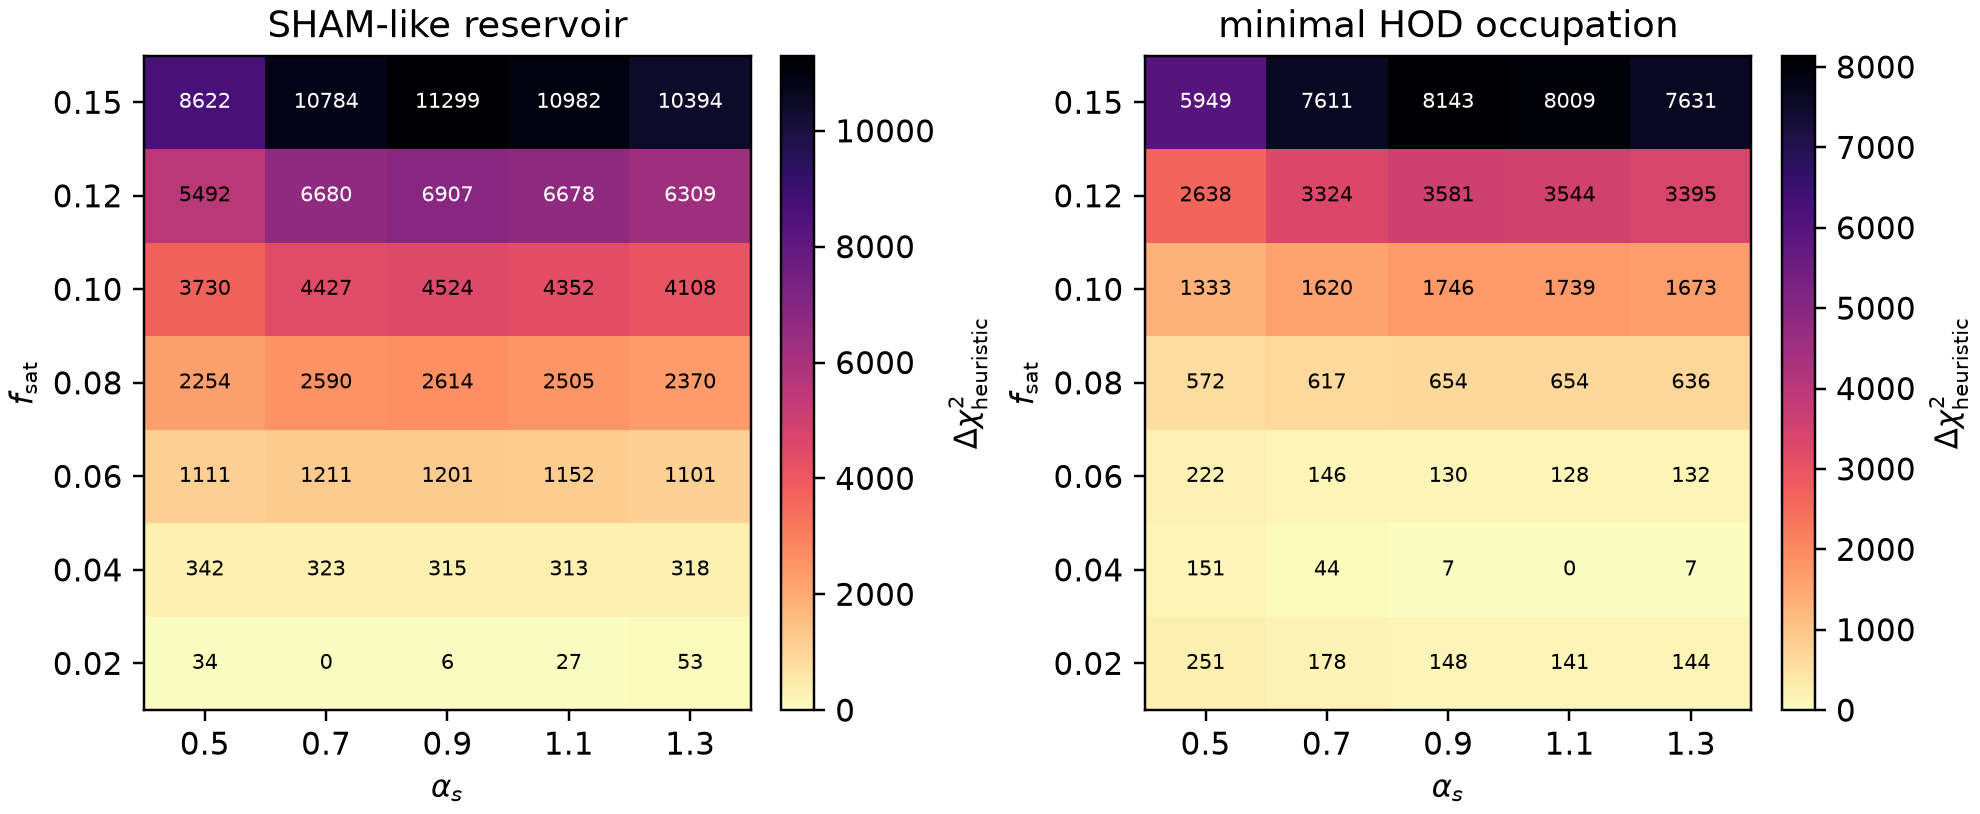
\includegraphics[width=0.86\textwidth]{figures/fig_extended_grid_heatmaps.png}
  \caption{Baseline extended SHAM-like and minimal-HOD grids.  Each cell shows $\Delta\chi^2_{\rm heur}$ relative to the best point, minimized over the plotted parameters.  The minimal-HOD occupation improves over the SHAM-like reservoir but still favours a low satellite fraction.}
  \label{fig:baselineheatmap}
\end{figure*}

The observable split explains the low-$\fsat$ preference.  The projected clustering $\wproj(r_{\rm p})$ penalizes high satellite fractions much more strongly than the large-scale multipoles.  In the minimal-HOD case, $\xizero+\xitwo$ with the full covariance can prefer a somewhat higher satellite fraction, while $\wproj$ pulls the joint solution back to low $\fsat$.

\subsection{Phenomenological radial dilution}

The direct radial-dilution test confirms that the satellite radial profile is a leading systematic.  Allowing $q$ in equation~(\ref{eq:qprofile}) improves the minimal-HOD heuristic score from the $q=1$ baseline $\chi^2_{\rm heur}=\BaseDilChi$ to $\chi^2_{\rm heur}=\BestDilChi$ at $\fsat=\BestDilFsat$, $\alphas=\BestDilAlpha$ and $q=\BestDilQ$.  Figure~\ref{fig:profiledilution} shows that increasing $q$ reduces the penalty for higher satellite fractions but does not make $\fsat=0.10$--0.12 competitive.

\begin{figure*}
  \centering
  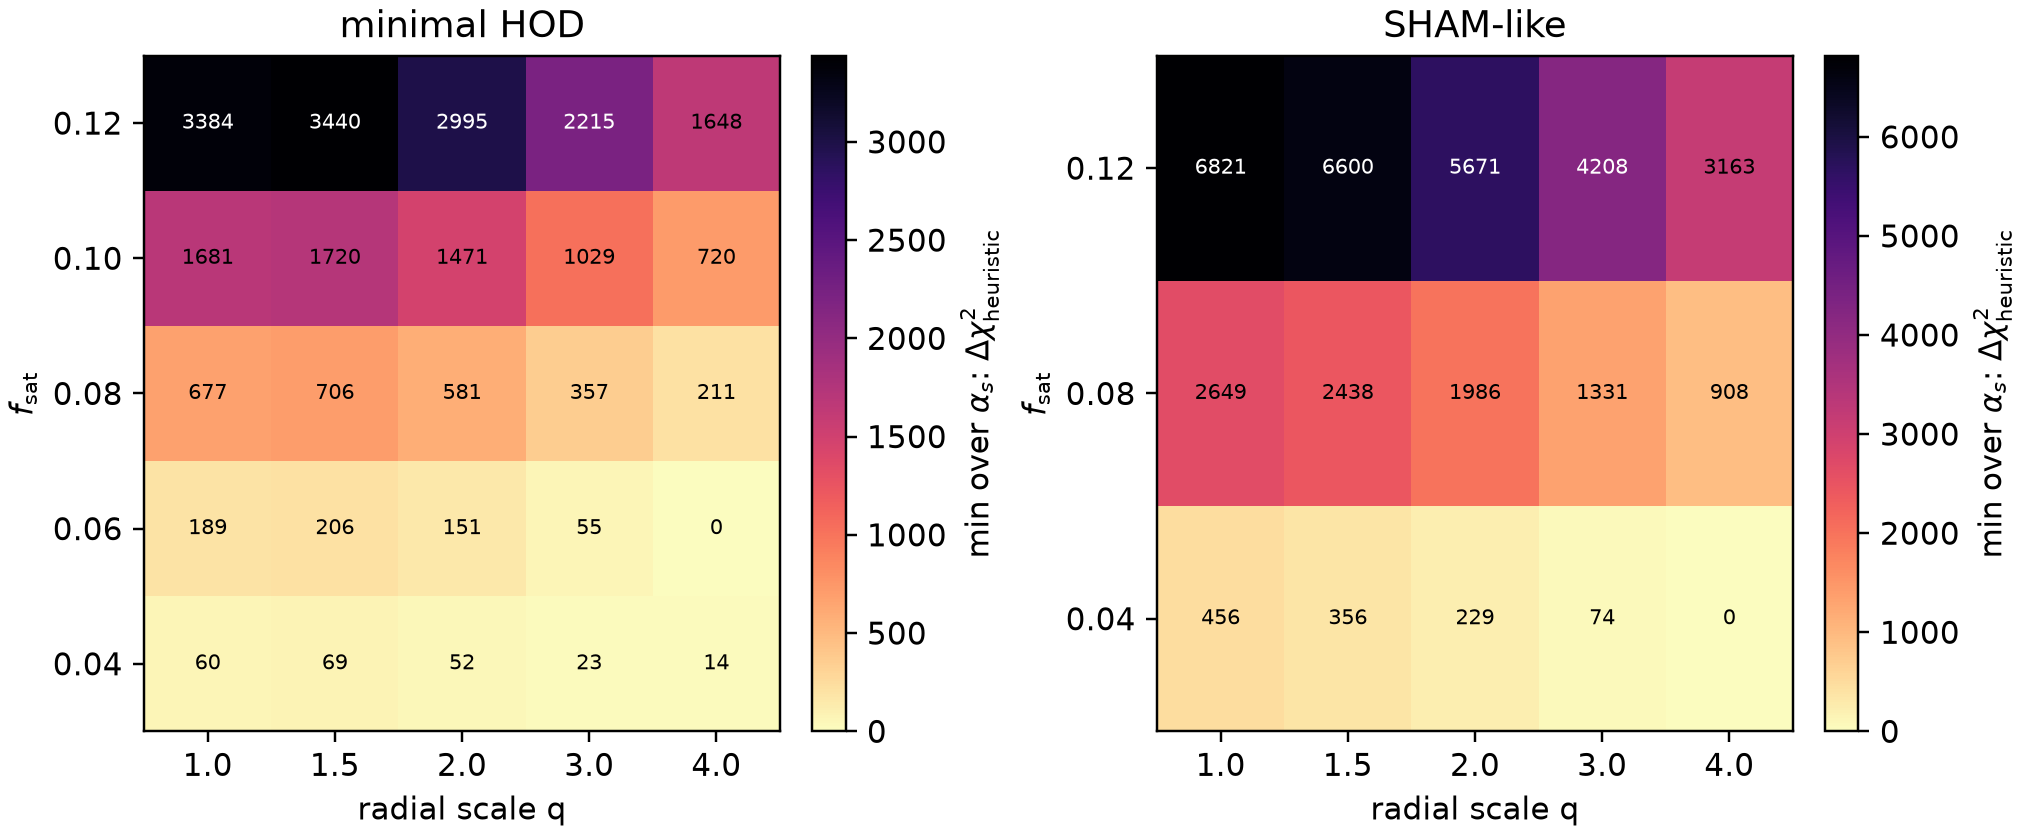
\includegraphics[width=0.86\textwidth]{figures/fig_profile_dilution_heatmaps.png}
  \caption{Radial-dilution test.  The direct scaling parameter $q$ lowers the small-scale $\wproj$ penalty and shifts the heuristic minimal-HOD best fit to $\fsat=0.06$, but high satellite fractions remain disfavoured.}
  \label{fig:profiledilution}
\end{figure*}

This behaviour is clearer in Fig.~\ref{fig:tradeoff}.  Increasing $q$ systematically reduces the $\wproj$ contribution for each satellite fraction.  The RSD quadrupole, however, does not respond in the same way.  This creates a trade-off: the model can reduce the small-scale projected excess, but it cannot freely move to high $\fsat$ without degrading the multipoles.

\begin{figure*}
  \centering
  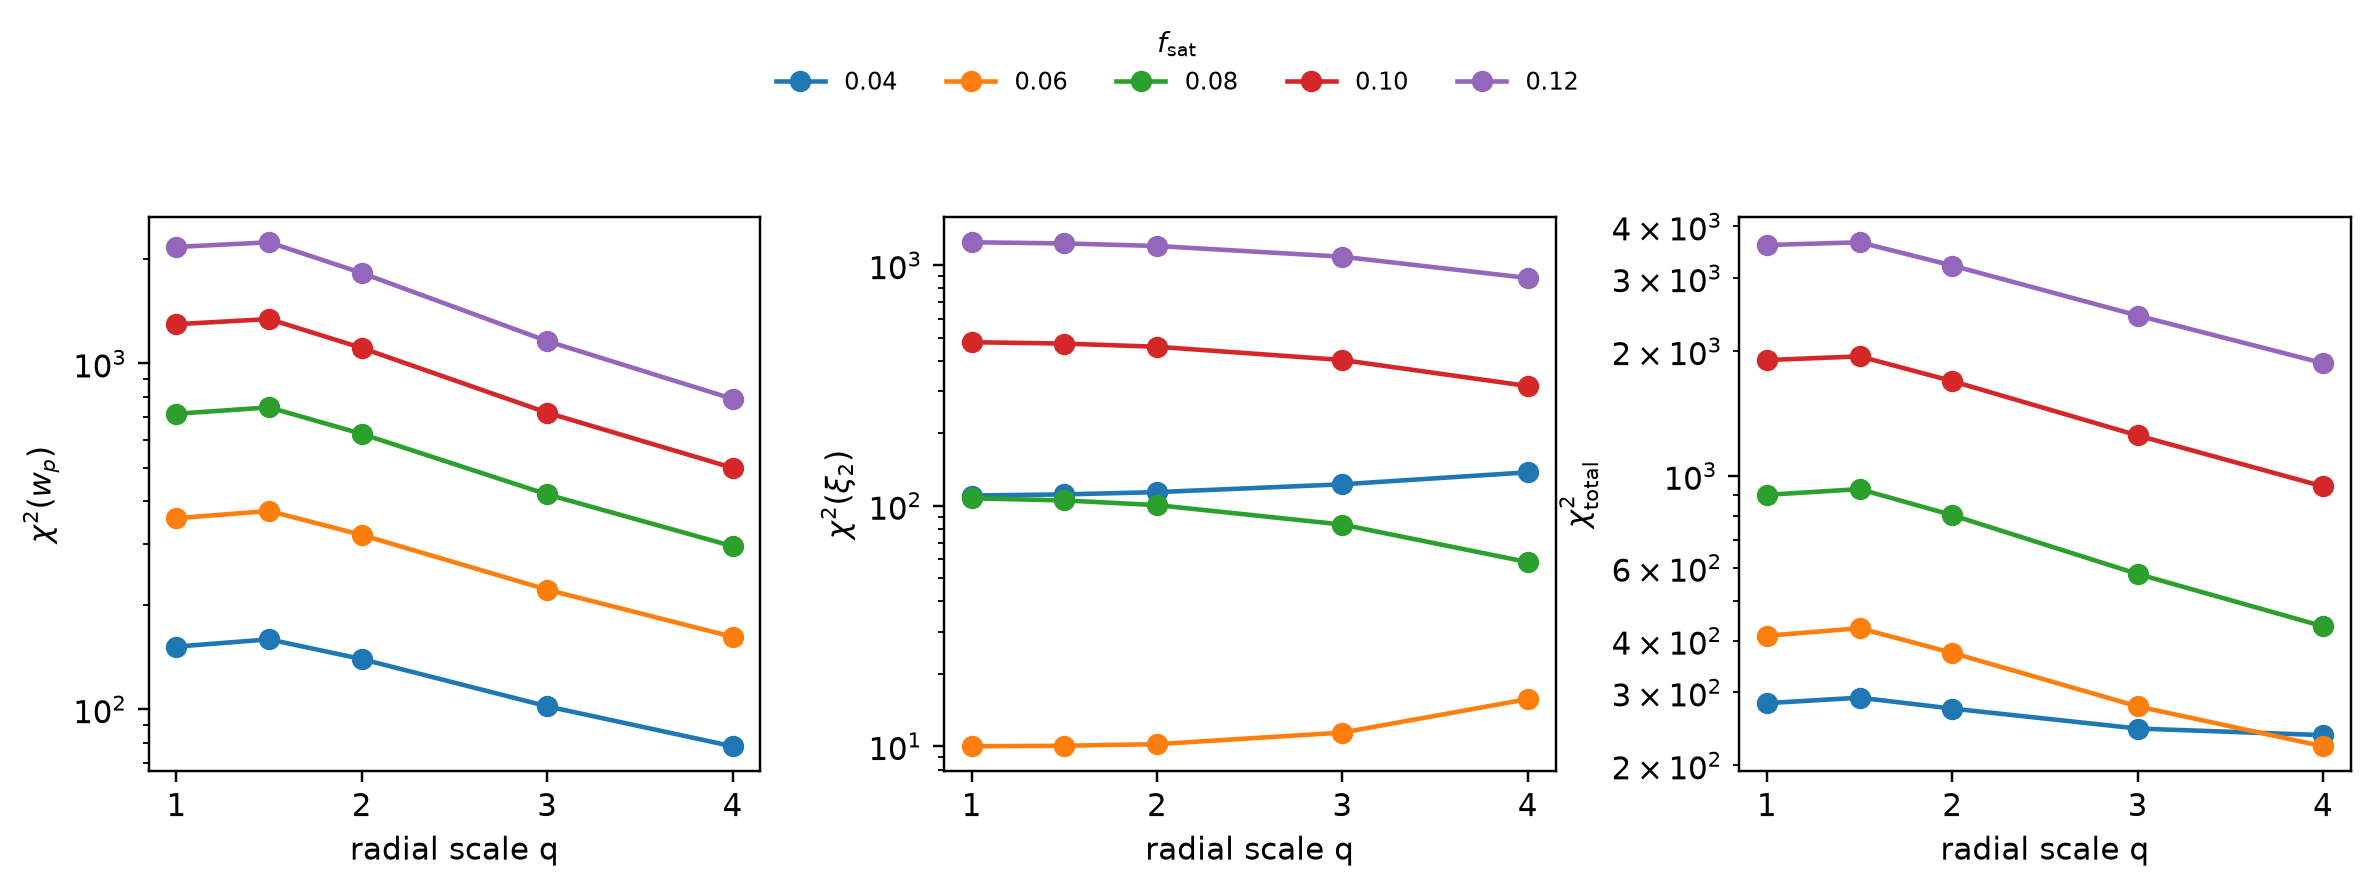
\includegraphics[width=0.95\textwidth]{figures/fig_profile_tradeoff.png}
  \caption{Observable trade-off in the minimal-HOD radial-dilution grid.  The main gain from increasing $q$ comes from $\wproj$, while the multipole contribution responds differently.  This split is the origin of the joint-fit tension.}
  \label{fig:tradeoff}
\end{figure*}

\begin{figure}
  \centering
  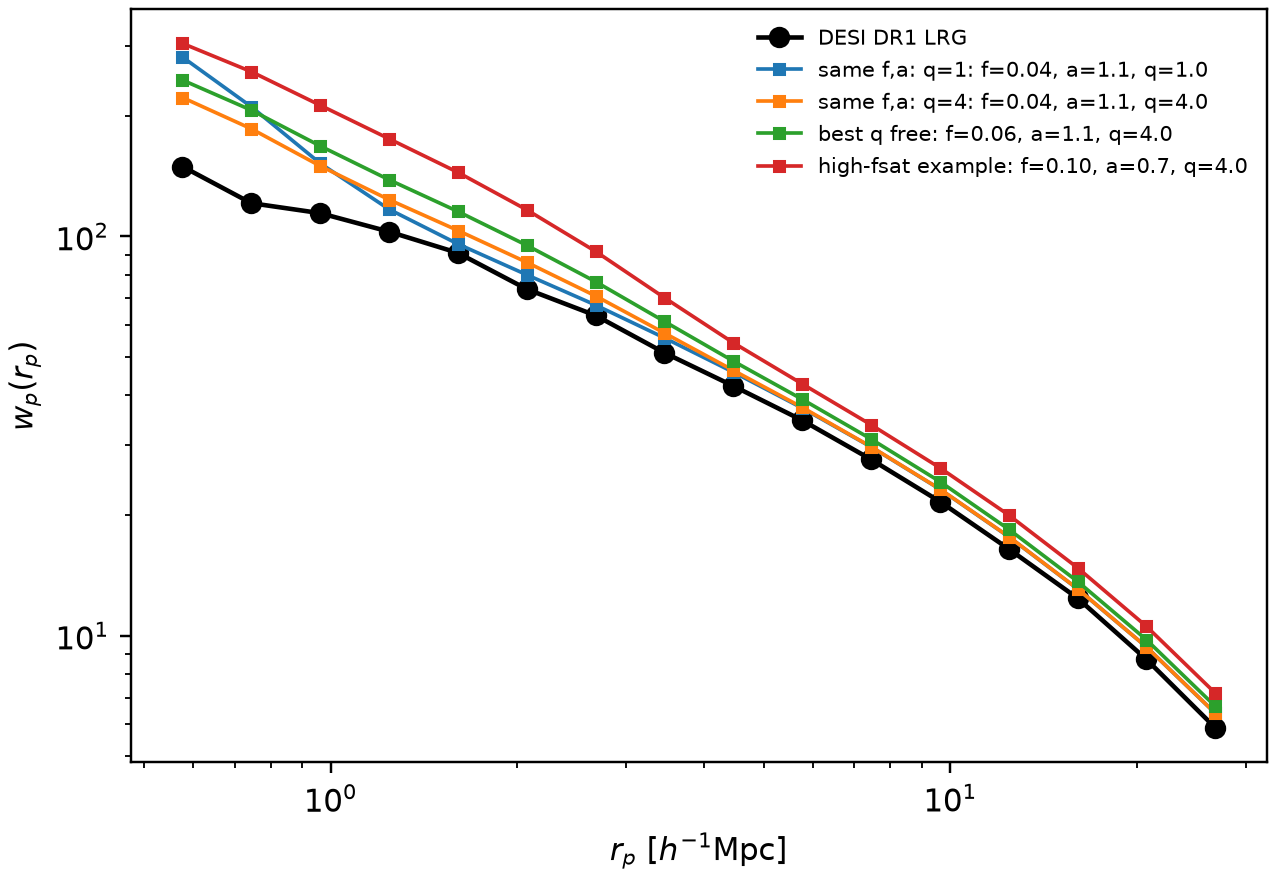
\includegraphics[width=\columnwidth]{figures/fig_wp_profile_curves.png}
  \caption{Projected clustering for selected minimal-HOD profile models.  The same-parameter $q=1$ and $q=4$ curves show directly how radial dilution changes the small-scale $\wproj$ mismatch.}
  \label{fig:wpcurves}
\end{figure}

The covariance-weighted split is more conservative than the heuristic score.  For the direct radial-dilution grid, the full joint covariance still selects $\fsat=0.04$ and $q=4$, while the heuristic score selects $\fsat=0.06$.  We interpret this not as a contradiction but as evidence that $\wproj$ and RSD multipoles are pulling in partially different directions in the simplified model.

\subsection{NFW concentration-remapping control}
\label{sec:nfwresults}

The NFW concentration-remapping grid provides a more physical counterpart to the direct $q$ scaling.  The best point is $\fsat=\BestNFWFsat$, $\alphas=\BestNFWAlpha$, and $c_{\rm ratio}=\BestNFWCratio$ ($c_{\rm sat}=\BestNFWCsat$), with $\chi^2_{\rm heur}=\BestNFWChi$.  Relative to the $c_{\rm ratio}=1$ baseline, $\chi^2_{\rm heur}=\BestNFWBaseChi$, this is only a modest improvement.  The remapping changes the satellite radii at fixed NFW quantile rather than applying an arbitrary linear dilation.

\begin{figure}
  \centering
  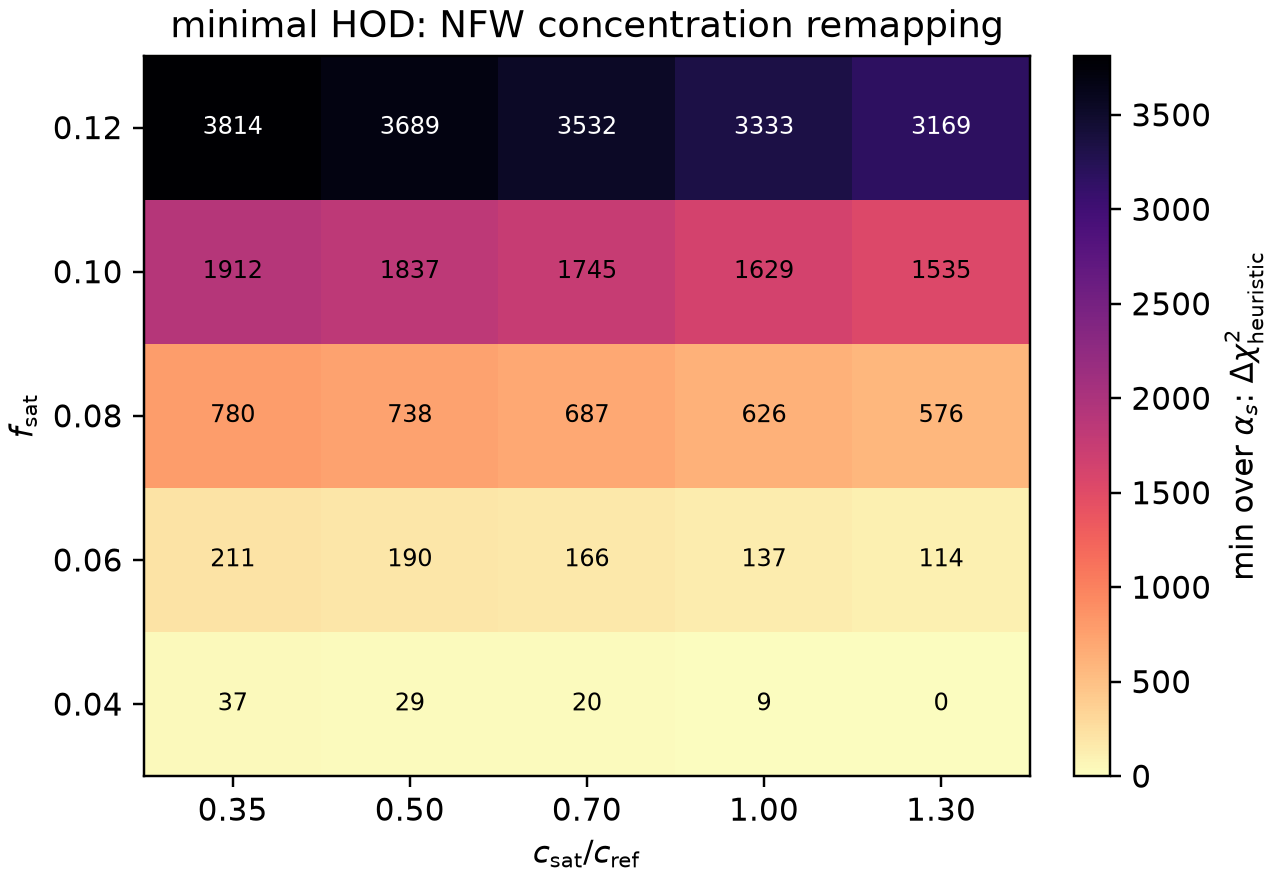
\includegraphics[width=\columnwidth]{figures/fig_nfw_profile_heatmap.png}
  \caption{NFW concentration-remapping control.  The plotted quantity is $\Delta\chi^2_{\rm heur}$, minimized over $\alphas$, as a function of target satellite fraction and concentration ratio $c_{\rm sat}/c_{\rm ref}$.  This physically motivated profile freedom tests whether a standard concentration change can reproduce the large improvement seen in the direct $q$-dilution experiment.}
  \label{fig:nfwprofile}
\end{figure}

The key point is that the NFW remapping does not erase the low-$\fsat$ tendency.  The best high-satellite rows at $\fsat=0.10$ and $0.12$ have $\chi^2_{\rm heur}=\BestNFWTenChi$ and $\BestNFWTwelveChi$, respectively, still far above the low-$\fsat$ solutions.  Thus, within this constrained NFW-family control, varying concentration alone is not sufficient to recover the $\fsat\simeq0.10$--0.15 region while also matching $\xizero+\xitwo$.

\section{Discussion}
\label{sec:discussion}

The strongest conclusion is not that DESI LRG clustering generically requires a very low satellite fraction.  Rather, in this public full-box compact-mock setup, the inferred $\fsat$ is highly sensitive to the satellite radial profile used by the simplified occupation model.  A model with too much one-halo projected power is driven toward low $\fsat$ by $\wproj(r_{\rm p})$, even if the redshift-space multipoles could accommodate a larger satellite contribution.

The main empirical signature is therefore not a uniform preference across the whole clustering vector.  The low-$\fsat$ preference is driven by $\wproj$, not by the full clustering vector uniformly.  In the split fits, small-scale projected clustering carries the strongest penalty against high satellite fractions, while $\xizero+\xitwo$ can move in a different direction once velocity bias and profile changes are allowed.  This observable dependence is the reason we interpret the result as a profile-systematics diagnostic rather than a direct physical measurement of the DESI LRG satellite fraction.

This conclusion also explains why the result should not be read as a contradiction of full AbacusHOD analyses.  DESI One-Percent AbacusHOD fits find $\fsat\simeq0.10$--0.14, consistent with broader BOSS/eBOSS LRG HOD expectations \citep{Yuan2022,Yuan2024,Zhai2017}.  Those analyses marginalize over richer occupations, assembly-bias or velocity-bias freedom, cleaned haloes, DESI-like selection and more realistic covariance treatment.  Our lower values are diagnostic preferences from a compact public-box reservoir.  The discrepancy is best read as evidence that an over-concentrated or otherwise mismatched satellite reservoir can force simplified fits toward artificially low $\fsat$.

The practical implication is that resource-limited mock analyses should split $\wproj$ from $\xizero+\xitwo$ and introduce at least one satellite-profile control before interpreting $\fsat$ astrophysically.  The remaining limitations are important: the covariance is a 96-region jackknife, the box is periodic, fibre assignment and imaging systematics are absent, and the minimal-HOD layer is deliberately simpler than AbacusHOD.  These choices are appropriate for a diagnostic Letter but not for a definitive DESI HOD inference.

\section{Conclusions}
\label{sec:conclusions}

We have used a public Abacus full-box compact catalogue to study the sensitivity of DESI LRG HOD inference to satellite fraction, velocity bias and satellite radial profile.  This is not a replacement for full DESI AbacusHOD inference, but a diagnostic study of satellite-profile systematics.  The main results are:

\begin{enumerate}
  \item SHAM-like and minimal-HOD samples both prefer low $\fsat$ in the baseline $\wproj+\xizero+\xitwo$ fit, with the minimal-HOD grid favouring $\fsat=\BestHODFsat$.
  \item The low-$\fsat$ preference is driven by small-scale $\wproj$, not by the full clustering vector uniformly.
  \item Direct radial dilution improves the heuristic minimal-HOD fit from $\chi^2=\BaseDilChi$ to $\chi^2=\BestDilChi$ and shifts the best point to $\fsat=\BestDilFsat$.
  \item NFW concentration remapping gives only a modest improvement, so ordinary concentration changes alone do not make $\fsat=0.10$--0.15 competitive.
\end{enumerate}

The next valuable step is a full joint inference of $\fsat$, $\alphas$ and satellite profile using an official AbacusHOD or equivalent model with DESI-like selection, fibre assignment and mock covariance.

\section*{Acknowledgements}

This work uses public AbacusSummit simulation products and DESI LRG clustering measurements.  The analysis was developed as a resource-limited pilot study using local Windows processing and ParaCloud cluster runs.  The author thanks Lehman Garrison for providing helpful information about the Abacus data source.  The author acknowledges support from the National Natural Science Foundation of China under Grant No. 11303079, and from Zhejiang Guangsha Vocational and Technological University of Construction under Grant No. 2022KYQD-KDB.

\section*{Data Availability}

The analysis scripts, lightweight summary tables, figure-generation products and manuscript source are available at \url{https://github.com/billkang-x/desi-lrg-satellite-profile-systematics}.  Large external catalogues and regenerated binary products are not included in the repository.  The AbacusSummit input products are publicly available from the AbacusSummit data release, and the DESI clustering measurements used here are public DESI DR1 LRG measurements or derived products from the same data vector.

\bibliographystyle{mnras}
\bibliography{references}

\label{lastpage}
\end{document}
